\documentclass[]{indojc_single}

\usepackage{times,amsmath}
\usepackage{amssymb}
\usepackage{graphicx}
\usepackage{lipsum}
\usepackage{url}
\usepackage{fixltx2e}
\usepackage{cite}
\usepackage{float}
\usepackage{algorithm}
\usepackage{algpseudocode}
\usepackage[T1]{fontenc}
\renewcommand{\refname}{Daftar Pustaka}
\usepackage[bahasa]{babel}
% correct bad hyphenation here
\hyphenation{op-tical net-works semi-conduc-tor}

\begin{document}

\makeatletter
\title{IoT on Heart Arrhythmia Real Time Monitoring}

%Please change "Sample Paper with indojc Class for Indonesian Journal on Computing" with your title bellow:
\newcommand{\Title}{\reverseit{IoT on Heart Arrhythmia Real Time Monitoring}}

\author{%
{Satria Mandala{\small $~^{*1}$}, \and Muhammad Alif Akbar{\small $~^{\#2}$}}%
\vspace{1.6mm}\\
\fontsize{10}{10}\selectfont\itshape
$^{*\#}$\,Department of Informatics Engineering, \\
School of Computing, Telkom University\\
Bandung, Jawa Barat, Indonesia\\
\fontsize{9}{9}\selectfont\upshape
$^{1}$\, satriamandala@telkomuniversity.ac.id\\
$^{2}$\, maakbar@student.telkomuniversity.ac.id%
}

%Please change "First Author" below into you paper's first author
\newcommand\Author{Muhammad Alif Akbar}


\maketitle
\thispagestyle{empty}
\pagestyle{empty}

%Please change "First Author" below into you paper's first author
\newcommand\Author{First Author}
\maketitle
\pagestyle{empty}

% As a general rule, do not put math, special symbols or citations
% in the abstract or keywords.
\def\abstractname{Abstract}
\def\keywordsname{Keywords}
\begin{abstract}
Heart monitoring is popular in the recent 5 yearns. We can see this with emergence of various cardiovascular monitoring products based on wearable sensors. Those products commonly communicates using radio telemetry which has expensive operational costs. Some research try to implement internet of things (IoT) concept to solve the issue. However, those IoT implementation aren't efficient enough. The research are only focused on how to read the sensors data and allowing it to be monitored on real-time. This research proposed a cloud based IoT architecture to monitor arrhythmia, one type of a common heart attack, which more efficient than previous research. Arrhythmia detector that used in this paper is an improvement of algorithm proposed by Tsipouras et al, which using R peak on ECG. The system proposed on this paper has been tested using MIT-BIH datasets and has result 93.11\% accuracy against 3 arrhythmia class, that is PAC, PVC and VT. The interesting result is that by implementing IoT, the R-Peak detection algorithm's execution time decreased up to 30\% compared to has been proposed by Pan and Tompkins. The average of execution time of every sample is decreased to 0.00749 ms.
\end{abstract}

\begin{keywords}
IoT, heart monitoring, Arrhythmia
\end{keywords}
$~$\\

% As a general rule, do not put math, special symbols or citations
% in the abstract or keywords.
\def\abstractname{Abstrak}
\def\keywordsname{Kata Kunci}
\begin{abstract}
Monitoring jantung telah populer sejak 5 tahun terakhir. Hal ini ditandai dengan munculnya berbagai produk monitoring jantung berbasis wearable sensor. Umumnya komunikasi yang digunakan pada sistem tersebut menggunakan radio telemetri dengan biaya operasional yang mahal. Beberapa riset mencoba menggunakan konsep internet of things (IoT) untuk mengatasi hal tersebut. Namun demikian, desain komunikasi IoT yang ada belum efisien. Ini disebabkan riset yang ada hanya berfokus pada bagaimana hasil baca sensor dapat dipantau secara realtime. Untuk mengatasi hal tersebut, riset ini mengusulkan sebuah arsitektur IoT berbasis cloud untuk memonitor aritmia, salah satu jenis penyakit jantung yang umum ditemukan. Deteksi aritmia yang diusulkan adalah pengembangan algoritma yang sebelumnya diusulkan oleh Tsipouras et al, dengan menggunakan deteksi fitur R dalam ECG. Sistem yang diusulkan pada paper ini telah diuji menggunakan dataset MIT-BIH dan menghasilkan akurasi 93.11\% terhadap 3 kelas aritmia, yaitu PAC, PVC dan VT. Menariknya, dengan penerapan IoT, efisiensi waktu eksekusi algoritma pendeteksi fitur R meningkat 30\% dibanding yang diusulkan oleh Pan dan Tompkins. Terbukti dengan rendahnya waktu rata-rata eksekusi tiap sampel data, yaitu sekitar 0.00749 ms.
\end{abstract}

\begin{keywords}
IoT, heart monitoring, Arrhythmia
\end{keywords}

\section{Pendahuluan}
\TSoCPARstart{B}{elakangan} ini monitoring jantung mendapatkan perhatian lebih dari publik. Hal ini terlihat dari bermunculannya produk \textit{wearable} yang memungkinkan monitoring jantung dimana saja dan kapan saja \cite{online:fitbit, online:samsung_gear, online:endo_holter}. Umumnya produk tersebut menggunakan \textit{electrocardiography} (ECG) ataupun \textit{photoplethysmography} (PPG) sebagai sensornya. Penggunaan ECG dapat ditemukan pada produk produk holter monitor \cite{online:endo_holter}. Penggunaan PPG dapat ditemukan pada produk produk jam tangan pintar seperti FitBit dan Gear Watch yang menambahkan PPG di bagian belakang jamnya \cite{online:fitbit, online:samsung_gear}. Sensor-sensor ini akan membaca sinyal jantung lalu menampilkan perkiraan jumlah detak jantung permenit (BPM) pada layar produk ataupun layar ponsel yang terhubung ke produk tersebut. Selain produk \textit{wearable} diatas, produk berupa software yang memanfaatkan kamera pada belakang ponsel juga banyak ditemukan pada \textit{online store} seperti \textit{android play store} \cite{playstore_heart}.

Beberapa penelitian telah dilakukan untuk menerapkan konsep IoT \cite{daniel_barataa, paola_pierleoni, vasu_jindal, mamidi}. Namun penelitian tersebut belum dapat memaksimalkan kemampuan yang ditawarkan oleh IoT. Kemampuan yang belum diterapkan seperti \textit{multi user monitoring, online recording, online analyzing, dan real time alerting}. Terlebih penelitian tersebut belum mempertimbangkan optimasi terhadap waktu pengiriman dan pemrosesan data. Penelitian tersebut hanya berfokus pada bagaimana hasil baca sensor dapat dipantau secara realtime oleh orang lain di tempat lain.

Pada paper ini kami merancang sebuah arsitektur IoT yang menerapkan deteksi aritmia pada \textit{cloud}. Deteksi aritmia yang diterapkan merupakan usulan algoritma oleh Tsipuras et al \cite{tsipouras} yang menggunakan fitur R pada ECG. Untuk mendeteksi fitur R, diterapkan modifikasi terhadap algoritma usulan Pan-Tompkins \cite{pantom}. Modifikasi yang dilakukan ditujukan untuk mengurangi waktu eksekusi yang diperlukan algoritma sehingga \textit{cloud} dapat melayani lebih banyak \textit{sensor}. Pembahasan tentang arsitektur monitoring aritmia berbasis iot yang diusulkan dapat dilihat pada bab \ref{section:bab2}. Bab \ref{section:bab3} menjelaskan tentang algoritma yang digunakan untuk mendeteksi terjadinya aritmia. Sedangkan Bab 4 mendiskusikan tentang pengujian sistem dan hasilnya.

\section{Arsitektur Monitoring Aritmia berbasis Internet of Things (IoT)} \label{section:bab2}
Sebuah sistem IoT umumnya memiliki 3 komponen yaitu \textit{Sensor}, \textit{Server} (selanjutnya disebut \textit{cloud}) dan \textit{Actuator}. Pada rancangan arsitektur di paper ini, tidak ada \textit{actuator} yang bersifat sebagai pelaksana suatu perintah. \textit{Actuator} yang diterapkan bersifat sebagai penerima pesan peringatan ketika terjadi aritmia dan modul untuk melakukan \textit{real time monitoring}, selanjutnya disebut \textit{dashboard}.

Secara umum sistem bekerja dimulai dari sebuah sensor membaca sinyal jantung seorang pasien. Kemudian sensor akan terkoneksi ke \textit{cloud} dan mengirimkan hasil bacanya secara periodik. Protokol komunikasi yang digunakan dalam sistem ialah MQTT. \textit{Cloud} akan memroses sampel dan mengirimkan hasil \textit{filtering} dan notifikasi terjadinya aritmia kepada dashboard. \textit{Dashboard} akan berkomunikasi dengan \textit{cloud} tentang sensor mana yang ingin dipantau. Gambaran ini dapat dilihat pada gambar \ref{fig:overall_diagram}.

\begin{figure}[htbp]
\centerline{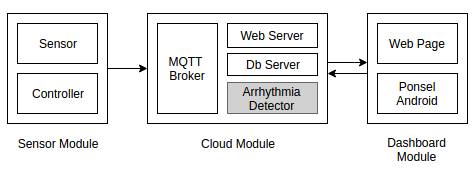
\includegraphics[scale=0.65]{images/overall.png}}
\caption{Diagram Rancangan Keseluruhan Sistem }
\label{fig:overall_diagram}
\end{figure}

\subsection{Sensor Module}
\textit{Sensor Module} dirancang hanya untuk membaca dan mangirimkan sinyal jantung, tidak ada pemrosesan berat pada modul. Hal ini ditujukan agar sensor dapat melakukan sampling dengan frekuensi yang tinggi. Selain itu, hal tersebut memungkinkan kedua jenis sensor (ECG atau PPG) dijadikan \textit{input} pada modul. 

Sensor yang dirancang melakukan \textit{sampling} pada 200Hz atau 5ms/sampel. Frekuensi sampel yang tinggi ini membutuhkan protokol komunikasi yang cepat sehingga sampel tidak memenuhi \textit{buffer} yang disediakan. Oleh karena itu, MQTT dipilih sebagai protokol komunikasi pada arsitektur yang dirancang. Setiap pesan dikirim menggunakan skema \textit{fire-and-forget} pada MQTT (MQTT-QOS 0). Namun, karena tidak ada jaminan sampel sampai pada \textit{cloud} maka perlu dilakukan penanganan data hilang. Hal ini dilakukan dengan memberikan index pada setiap sampel yang dikirim. Index ini akan direset setiap 1000 sampel untuk meminimalkan penggunaan memori pada modul dan mengurangi ukuran paket yang dikirim.

\subsection{Cloud Module}
Semua pemrosesan dilakukan di \textit{cloud/server}. \textit{Cloud} bekerja dengan membagi pekerjaan kepada unit-unit proses. Sebuah unit proses secara khusus menangani sebuah sensor dengan suatu ID unik. Sistem membuat unit proses ketika sebuah ID baru saja terhubung dan menutupnya ketika ID tersebut berhenti terhubung. 

Sebuah unit proses akan memproses sampel berdasarkan index yang menyertai sampel tersebut. Ketika terdeteksi index yang hilang maka akan dilakukan penanganan data yang hilang. Index dikatakan hilang jika terjadi lompatan index yang diterima, misalnya proses menanti index bernomor 5 namun yang diterima ialah index bernomor 10. Penanganan data yang dilakukan ialah menghitung berapa nilai yang hilang berdasarkan garis lurus dari nilai sampel terakhir yang diterima ke nilai sampel sebelumnya (persamaan \ref{eq:line}). Nilai sampel ini, baik yang asli ataupun hasil perkiraan akan disimpan dalam \textbf{database} pada server.

\begin{equation}
y(n) = \dfrac{n (v_{2} - v_{1})}{d} + v_{1}
\label{eq:line}
\end{equation}

$v_{1}$ adalah nilai terakhir yang diterima, $v_{2}$ adalah nilai terbaru yang diterima, $n$ adalah jarak dari index terakhir, $d$ adalah jarak index terbaru ke terakhir. $y$ adalah nilai index $n$ yang hilang

Sampel kemudian diproses untuk dilakukan \textbf{filtering}, \textbf{r-peak detection}, dan klasifikasi aritmia. Sampel yang telah difilter akan divisualisasika pada \textbf{dashboard}. Karena frekuensi sampel yang diterima sangat tinggi maka perlu dilakukan \textbf{downsample} terhadap data sampel tersebut sebelum dapat divisualisasikan pada sebuah monitor. Nilai frekuensi downsampel yang dipilih ialah 20Hz (20 FPS), nilai umum frekuensi sampel banyak monitor yang ada dipasaran.

\subsection{Dashboard Module}
Dashboard berfungsi sebagai penerima pesan peringatan dan modul pemantauan. Dengan menerapkan MQTT pada rancangan arsitektur, hubungan antara modul \textit{sensor-cloud-dashboard} dapat digambarkan sebagai pola \textbf{subscriber} dan \textbf{publisher}. Hal ini memungkinkan banyak \textbf{dashboard} untuk \textbf{subscribe} kepada ID sensor. Sekaligus memungkinkan dikirimnya \textit{push notification} kepada semua \textbf{dashboard} tersebut ketika sebuah ID yang dipantau mengalami serangan aritmia, yang dapat berupa ponsel android maupun halaman web.
\section{Pendeteksi Aritmia} \label{section:bab3}
Telah banyak penelitian dilakukan untuk mengklasifikasikan aritmia berdasarkan sinyal ECG. Terdapat metode klasifikasi yang memanfaatkan metode kecerdasan buatan seperti \textit{support vector machine} (SVM) \cite{aritmia_svm} dan \textit{Artificial Neural Network} (ANN) \cite{aritmia_ann}, ada pula yang memanfaatkan aturan yang dibuat oleh dokter ahli jantung \cite{tsipouras}. Pada arsitektur yang dirancang diterapkan klasifikasi yang memanfaatkan aturan yang dibuat oleh ahli jantung. Aturan ini pertama kali diusulkan oleh Tsipouras et al, pada percobaan mereka menghasilkan akurasi yang cukup tinggi dibandingkan dengan algoritma yang lebih kompleks \cite{tsipouras}.

Algoritma \textit{Arrhythmia Detector} akan berjalan pada server (lihat gambar \ref{fig:overall_diagram}, diberi warna abu). Deteksi aritmia terbagi menjadi 2 tahap yaitu \textit{R-Peak detection} dan \textit{Arrhythmia detection}. \textit{R peak detection} bertujuan untuk menemukan gelombang R pada sinyal ECG. Lalu \textit{R peak} ini akan menjadi inputan pada \textit{Arrhythmia detection}. Deteksi puncak R dilakukan dengan memanfaatkan modifikasi terhadap metode yang diajukan oleh Pan-Tomkins.

\subsection{Deteksi Puncak R oleh Pan and Tompkins}
Pan dan Tompkins mengusulkan sebuah algoritma pencarian QRS pada sinyal ECG \cite{pantom}. Metode ini menjadi populer karena dapat bekerja secara \textit{real-time}. Metode PanTomkins dimulai dari proses \textit{preprocessing} berupa filtering sinyal. Kemudian dilanjutkan dengan pencarian puncak R menggunakan \textit{adaptive thresholding}. 

Pada tahap \textit{preprocessing}, Pan-Tompkins menerapkan 4 proses \textit{filtering} yaitu \textit{Band Pass filtering, Derived filter, Squaring}, dan \textit{Moving Window Integrator} (MWI), seperti yang ditunjukkan pada gambar \ref{fig:preprocessing}. Tahapan tersebut dilakukan untuk menghilangkan \textit{noise} pada sinyal dan memudahkan proses pencarian puncak. 

Setelah tahap \textit{preprocessing}, dilanjutkan tahap \textit{processing}, Pan-Tompkins menerapkan \textit{adaptive thresholding} terhadap sebuah \textit{window} sinyal yang berukuran kecil (0.3s) \cite{pantom}. Pada \textit{window} tersebut, akan dicari \textit{peak} yang melewati threshold yang telah ditentukan, kemudian nilai peak akan menjadi input untuk  mengupdate nilai \textit{threshold}. Ketika sekian waktu terlampaui tanpa ditemukannya peak maka harus dilakukan search back hingga posisi R terakhir yang ditemukan (gambar \ref{fig:processing_ori}).

\begin{figure}[htbp]
\centerline{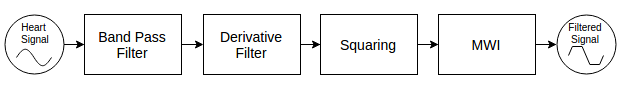
\includegraphics[scale=0.65]{images/preprocessing.png}}
\caption{Preprocessing: Filtering}
\label{fig:preprocessing}
\end{figure}

\begin{figure}[htbp]
\centerline{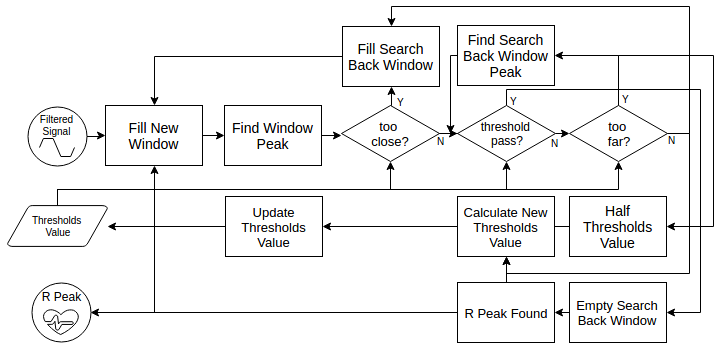
\includegraphics[scale=0.6]{images/processing_ori.png}}
\caption{Processing: Original R Peak Detection}
\label{fig:processing_ori}
\end{figure}

\subsection{Modifikasi Algoritma Pan - Tompkins dalam Deteksi Puncak R}
Penulis melihat algoritma Pan-Tompkins dapat dioptimasi sehingga dapat bekerja lebih cepat. Optimasi dilakukan dengan mempebesar window sehingga mengurangi jumlah eksekusi yang perlu dilakukan dalam waktu yang sama, membuat threshold berdasarkan nilai rata-rata window tersebut, menghapus \textit{false beat} dengan menolak R yang terlalu dekat berdasarkan rata rata jarak R (gambar \ref{fig:processing_modif}). Pelebaran window berakibat pada meningkatnya \textit{delay} atas munculnya hasil deteksi sejak diterimanya sampel namun dapat meningkatkan akurasi deteksi.

\begin{figure}[htbp]
\centerline{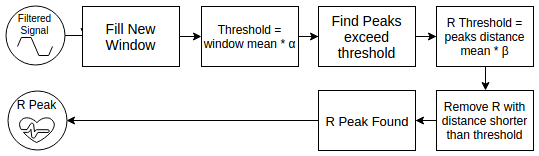
\includegraphics[scale=0.65]{images/processing_modif.png}}
\caption{Processing: Original R Peak Detection}
\label{fig:processing_modif}
\end{figure}

Nilai $\alpha$, $\beta$ serta lebar window yang diterapkan pada algoritma modifikasi didapatkan melalui hasil percobaan.

\subsection{Arrhythmia Detection}
Tsipouras et al. mengusulkan algoritma deteksi setelah melakukan percobaan bersama dokter spesialis jantung \cite{tsipouras}. Jenis aritmia yang dapat dideteksinya dibagi menjadi 4 jenis detak aritmia dan 7 jenis ritme aritmia. Namun untuk rancangan pada paper ini artimia yang dapat dideteksi hanyalah jenis aritmia detak dan dikelompokkan kedalam 3 kategori. Kategori yang dipilih ialah 1) Normal, 2) Premature Contraction, dan 3) Ventricular Flutter. Secara detil pengelompokan ini dapat dilihat pada tabel \ref{table:beat_classification}.

\begin{table}[!h]
	\begin{center}
	\caption{Arrhythmia Beat Classification}
	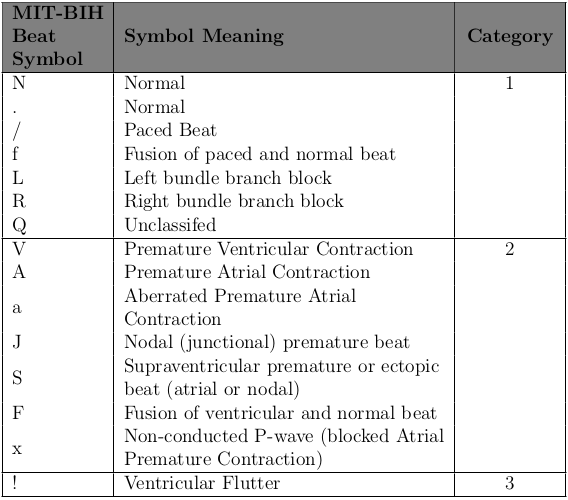
\includegraphics[scale=0.35]{images/class.png}	
	\label{table:beat_classification}
	\end{center}
\end{table}

Algoritma Tsipouras melakukan klasifikasi berdasarkan sebuah window RR interval yaitu $RR1_i$, $RR2_i$, dan $RR3_i$ yang kemudian seterusnya bergeser satu beat. RR interval merupakan jaruk waktu antar puncak R dalam satu detak. Tiap beat mulanya dikategorikan sebagai kelas 1 dan kemudian mendapatkan kategori baru sesuai \textit{Rule} yang telah ditetapkan (gambar \ref{fig:flowchart_aritmia}).
\\
\\
Rule 1. VF: Dimulai ketika $RR1_i > 1.8RR2_i$ dan durasi $RR2_i$ lebih kecil daripada 0.6 s. Maka $RR2_i$ dianggap sebagai awal mula terjandinya VF dan window berikutnya akan dites dengan kedua kondisi berikut:

\begin{enumerate}
	\item durasi setiap RR interval dalam satu window lebih kecil dari 0.7s
	\item jumlah durasi setiap RR interval dalam satu window lebih kecil dari 1.7s
\end{enumerate}

Jika salah satu kondisi tambahan pada rule 1 terpenuhi minimal 4 window berurutan maka RR2 pada tiap window tersebut diklasifikasikan sebagai beat kategori 3. Jika tidak algoritma berlanjut dan window kembali ke posisi awal ditemukannya VF.
\\
\\
Rule 2. PVC: Detak dikategorikan sebagai PVC jika salah satu kondisi berikut terpenuhi:

\begin{enumerate}
	\item $RR1_i > 1.15RR2_i$ dan $RR3_i > 1.15RR2_i$
	\item $|RR1_i - RR2_i| < 0.3s$ dan $RR1_i < 0.8s$ dan $RR2_i < 0.8s$ dan $1.2(RR1_i + RR2_i)/2 < RR3_i$
	\item $|RR2_i$ - $RR3_i| < 0.3s$ dan $RR2_i < 0.8s$ dan $RR3_i < 0.8s$ dan $1.2(RR2_i + RR3_i)/2 < RR1_i$
\end{enumerate}

\begin{figure}[htbp]
\centerline{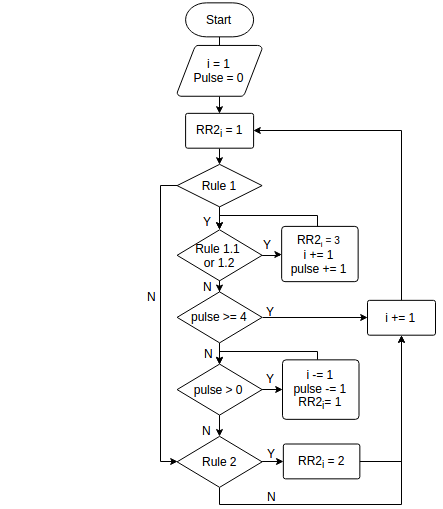
\includegraphics[scale=0.55]{images/flowchart_aritmia.png}}
\caption{Flowchart of Beat Aritmia Classification}
\label{fig:flowchart_aritmia}
\end{figure}

\section{Evaluasi Performansi}
Untuk menguji performa rancangan aristektur, rancangan arsiterkur perlu untuk diterapkan. Modul sensor diterapkan menjadi bentuk gelang tangan yang ditanamkan sensor berjenis PPG. ESP-12E lalu dipilih sebagai \textit{controller}-nya. ESP-12E dipilih karena bentuknya yang kecil dan spesifikasinya yang telah memiliki modul Wi-Fi. PPG dipilih hanya untuk mensimulasikan transmisi sinyal jantung, akurasi deteksi akan diukur menggunakan dataset ECG yang telah disedikan oleh MIT-BIH \cite{mit_bih_paper, physionet}. Modul cloud diterapkan secara lokal pada komputer ASUS K432SD@2.1GHz-RAM 6GB. Cloud akan diuji menggunakan 2 buah bahasa pemograman yang populer dalam membangun sistem IoT, yaitu Node.Js dan Python yang keduanya terhubung dengan database No-SQL MongoDb. Dashboard modul diterapkan menjadi sebuah halaman web dan menjadi sebuah aplikasi pada ponsel android.

Pengujian dilakukan oleh satu orang yang mengenakan modul sensor dan bergerak secara bebas dalam daerah yang tercakup WiFi. Modul sensor, Router WiFi dan \textit{Cloud} modul masih berada dalam satu wilayah yang sama sehingga diasumsikan tidak ada delay akibat proses \textit{routing}. Sehingga ketika terdeteksi artimia, dashboard modul dapat segera menerima push notifikasi dari MQTT. Namun karena keterbatasan maksimum FPS yang dapat dirender oleh monitor, sampel 200Hz harus di downsample hingga 20Hz pada dashboard.

\subsection{Waktu Eksekusi}
Setalah diuji, waktu eksekusi ditemukan cukup kecil. Waktu eksekusi mencakup diprosesnya sampel hingga menghasilkan deteksi aritmia (tahapan \textit{filter, save, detect}). Waktu eksekusi tercatat sebesar 0.00749 ms/sampel dengan menggunakan backend Node.JS dan 0.00991 ms/sampel dengan menggunakan backend Python. Ditemukan untuk rancangan arsitektur ini penggunaan nodejs lebih baik karena dengan alogritma dan spesifikasi server yang sama node.js dapat bekerja lebih cepat hingga 13\% daripada python.

Modifikasi algoritma deteksi R juga menghasilkan performa yang diharapkan ($\alpha = 1.1; \beta = 0.8; window = 6.5s$). Modifikasi algoritma menghasilkan waktu eksekusi hingga 30\% lebih cepat dari algoritma asli PanTompkin (gambar \ref{fig:exec_time}). Perbandingan hasil waktu eksekusi lengkap variabel dengan algoritma original dapat dilihat pada tabel \ref{table:beat_detection}.

\begin{figure}[htbp]
\centerline{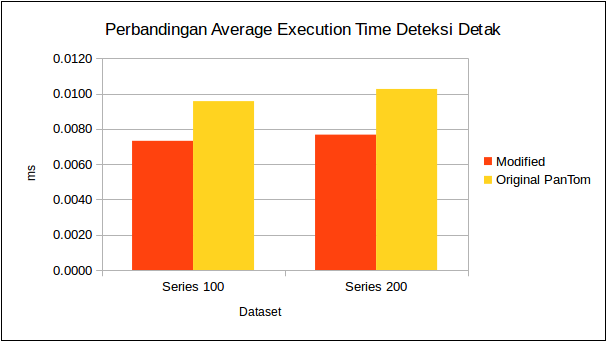
\includegraphics[scale=0.41]{images/beat_exec.png}}
\caption{Execution time comparison}
\label{fig:exec_time}
\end{figure}

\subsection{Deteksi}
Selain menghasilkan waktu eksekusi yang lebih cepat, modifikasi terhadap algoritma pantomkin juga memiliki tingkat akurasi yang menyamai algoritma pantomkin yang asli (gambar \ref{fig:beat_perform}). Perbandingan lengkap performa deteksi algoritma original dengan modifikasi dapat dilihat pada tabel \ref{table:beat_detection}.

\begin{table}[H]
	\begin{center}
	\caption{Hasil Pengujian Performa Deteksi Detak}
	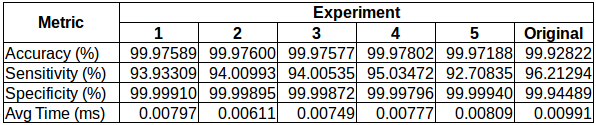
\includegraphics[scale=0.6]{images/beat_detection.png}	
	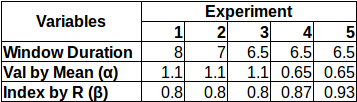
\includegraphics[scale=0.5]{images/experiment_variable.png}		
	\label{table:beat_detection}
	\end{center}
\end{table}

\begin{figure}[H]
\centerline{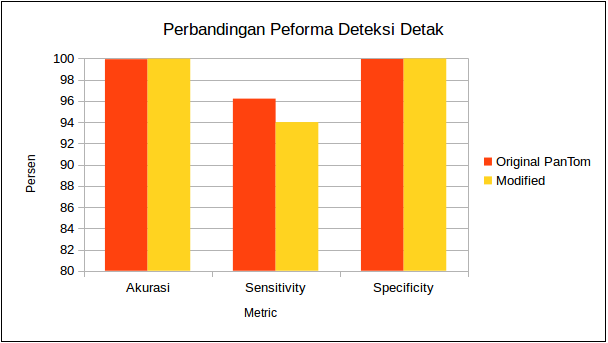
\includegraphics[scale=0.41]{images/beat_perform.png}}
\caption{Perbandingan Performa Deteksi Detak}
\label{fig:beat_perform}
\end{figure}

Dengan menerapkan algoritma deteksi aritmia usulan Tsipouras, sistem berhasil mendeteksi 3 kelas detak dengan performa akurasi yang cukup baik yaitu 93.11\% (gambar \ref{fig:aritmia_acc}). Perbandingan lengkap performa deteksi algoritma original dengan modifikasi dapat dilihat pada tabel \ref{table:aritmia_detection}. \textit{True Beat} adalah input posisi R asli dari dataset MIT-BIH.

\begin{table}[H]
	\begin{center}
	\caption{Hasil Pengujian Performa Deteksi Aritmia}
	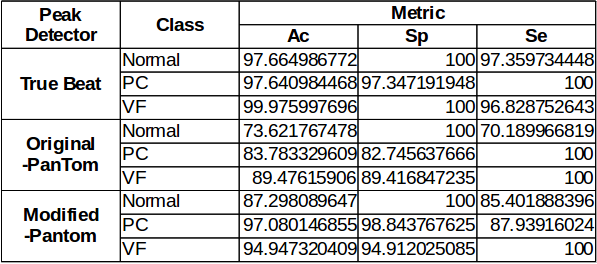
\includegraphics[scale=0.55]{images/aritmia_detection.png}	
	\label{table:aritmia_detection}
	\end{center}
\end{table}

\begin{figure}[H]
\centerline{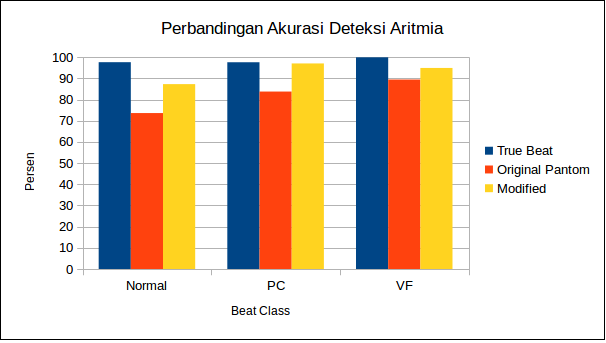
\includegraphics[scale=0.41]{images/aritmia_acc.png}}
\caption{Perbandingan Performa Deteksi Aritmia}
\label{fig:aritmia_acc}
\end{figure}

\section{Kesimpulan}
Monitoring aritmia jantung secara realtime menggunakan IoT berhasil dilakukan pada rancangan arsitektur, terlihat dari hasil akurasi deteksi yang mencapai 93.11\%. Yang menjadi perhatian utama dalam rancangan ini ialah bagaimana melakukan optimasi terhadap \textit{resource} yang terlibat, sehingga memungkinkan semakin banyak \textit{sensor} dan \textit{dashboard} yang dapat terhubung. Pilihan optimasi yang dapat dilakukan terdapat pada pemilihan bahasa \textit{server}, \textit{database}, hingga algoritma. Dengan menerapkan optimasi pada algoritma deteksi detak rancangan arsitektur dapat menangani hingga 1.4 kali labih banyak sensor (waktu eksekusi berkurang hingga 30\%). Penerapan algoritma yang lebih akurat dan mampu mendeteksi lebih banyak kelas dapat menjadi penelitian lanjutan yang menarik.

%Use following code if you use bibtex

\bibliographystyle{plain}
\bibliography{References}{}

\end{document}